\documentclass[a4paper,11pt]{article}

% Identificação
\newcommand{\rttitulo}{Do Arduino ao Banco de Dados \\ SQL ou NoSQL}
\usepackage{sty/iesb}

%----------------------------------------------------------------------
% Início do Documento
%-----------------------------------------------------------------------
\begin{document}

\thispagestyle{firstpage}
\begin{center}
	\hfill \break
	{ \huge \bfseries \rttitulo} \\[0.2 cm]
	Fernando Antonio Fernandes Anselmo - Versão 2.0
	\rule{\linewidth}{0.2 mm} \\[0.4 cm]
\end{center}

\section*{Introdução}
Nesta apostila vamos aprender como obter dados de sensores do mundo real, mas especificamente um sensor de Luminosidade juntamente com de temperatura, esse projeto possui um custo extremamente reduzido e o único componente "com um custo mais elevado" seria o \textbf{Arduino Uno} que pode ser reduzido com uma substituição por um \textbf{Arduino Micro} (que possui o custo bem mais acessível). Porém a compra do Uno é uma boa aquisição para qualquer Maker que se interesse por prototipação de projetos eletrônicos.

Como fonte de dados utilizaremos os cinco bancos a seguir:
\begin{figure}[H]
	\centering
	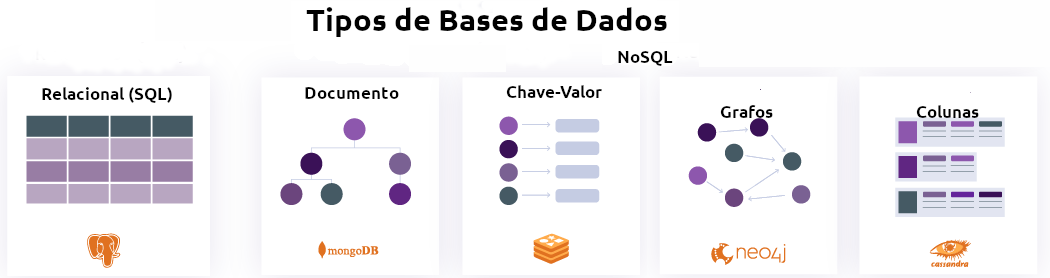
\includegraphics[width=0.8\textwidth]{images/NoSQL}
	\caption{Bancos de Dados utilizados}
\end{figure}

Utilizaremos no padrão SQL os SGBDR mais conhecidos do mercado \textbf{MySQL} e \textbf{Postgres}, além disso, alternativamente quatro NoSQL: \textbf{MongoDB} representando o tipo orientado a Documento, \textbf{Redis} orientado a Chave-Valor, \textbf{Neo4j} orientado a Grafo e \textbf{Apache Cassandra} orientado a Coluna, vai ser uma experiência interessante e comparativa pois podemos assim definir qual desses se encaixa melhor em um projeto que pretendemos realizar. Lembre-se apenas que ideia não é julgarmos, mas como característica comparativa e de aprendizado, pois cada banco de dados possui suas forças e fraquezas.

Para realizar o trabalho de intermediário (ou seja) quem lerá os dados da serial e enviará para o banco de dados será a linguagem Python. Essa é conhecida por sua simplicidade e facilidade de uso. Usaremos a porta serial como meio de obtermos os dados, assim é necessário instalar a biblioteca \textbf{PySerial}: \\
{\ttfamily\$ pip install pyserial}

E o padrão JSON para essa passagem, devemos também instalar a biblioteca \textbf{SimpleJson}: \\
{\ttfamily\$ pip install simplejson}

\section*{Montagem do Projeto}
Começamos com a montagem do projeto. Como entrada de dados usamos um componente chamado de \textit{Photoresistor} ou simplesmente \textbf{LDR} (abreviatura para \textit{Light Dependent Resistor}), isso é uma fotocélula e funciona como um resistor que varia com a intensidade de luz, quanto mais luz, mais alta é a resistência. Em conjunto um sensor de temperatura que também é conhecido como \textbf{LM35}. O preço de ambos não passa de poucos reais em qualquer casa de eletrônica.

Lista de componentes do projeto:
\begin{itemize}[nolistsep]
	\item 1 Arduino Uno Rev 3
	\item 1 LDR
	\item 1 LM35
	\item 1 Resistor de 1 K$\Omega$
	\item 6 jumpers para as conexões
	\item 1 micro protoboard (ou qualquer outra similar)
\end{itemize}

As conexões são realizadas conforme a seguinte figura:
\begin{figure}[H]
	\centering
	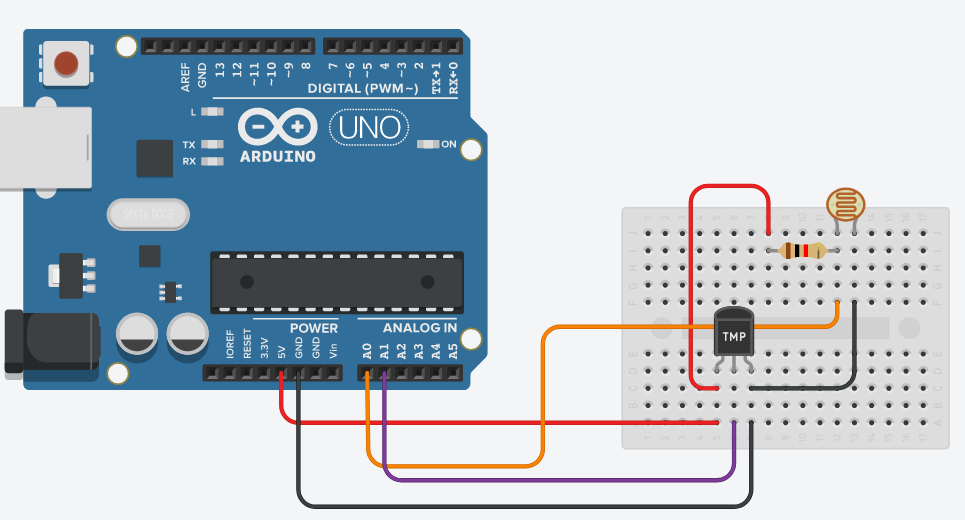
\includegraphics[width=0.60\textwidth]{images/circuito}
	\caption{Circuito da Ligação}
\end{figure}

Em uma de suas pernas do \textbf{LDR}, ligamos um \textit{jumper} para fazermos uma ponte para a GND do \textbf{LM35}, a outra perna possui uma dupla ligação: um \textit{jumper} para porta analógica \textbf{A0} e um resistor de 1 K$\Omega$ ligado em 5V como outra ponte para a alimentação do \textbf{LM35}. 

O componente \textbf{LM35} possui 3 pernas, para saber quais são o lado achatado desse sensor deve estar virado para nossa frente: a perna mais esquerda é ligada por um \textit{jumper} a alimentação de 5V, a central um \textit{jumper} para a porta analógica \textbf{A1} e a perna mais direita um \textit{jumper} para a \textbf{GND}.

Para a programação no Arduino, faremos a seguinte codificação:
\begin{lstlisting}[]
#define LDR A0
#define LM35 A1

int lums = 0;
float tensao;
float grauC;
float grauF;

void setup() {
  pinMode(LDR, INPUT);
  pinMode(LM35, INPUT);
  Serial.begin(9600);
}

void loop() {
  lums = map(analogRead(LDR), 244, 1100, 0, 100);
  tensao = (float(analogRead(LM35))*5)/1023; // 5V e leitura analógica 0 a 1023
  grauC = tensao / 0.010; // 0,010 mV
  grauF = grauC * (9.0/5.0) + 32.0;
  Serial.println("{\"lums\":" + String(lums) + ", \"grauC\":" 
  	+ String(grauC) + ", \"grauF\":" + String(grauF) + "}"); 
  delay(5000); // 5 segundos
}
\end{lstlisting}

Definimos uma constante \textbf{LDR} que aponta para a porta \textbf{A0} e outra \textbf{LM35} a porta \textbf{A1}. Definimos uma variável inteira chamada \textbf{lums} e três flutuantes que respectivamente conterão o valor da tensão, graus em Celsius e Fahrenheit. No método \textit{setup()} definimos as portas dos sensores como saída e iniciamos a serial na velocidade de \textbf{9.600 bounds} (isso é muito importante).

No método loop() obtemos a informação do componente que varia entre 244 a 1.100, porém para ficar mais "harmônico" criamos um mapa de valores que converte esse intervalo entre 0 a 100. Para obtermos o valor da temperatura primeiro calculamos a tensão, este sensor trabalha a 5V em uma porta analógica que varia de 0 a 1023. Basta agora dividir a informação por 0,010 que teremos o valor em graus \textit{Celsius}. E a partir dessa aplicamos uma fórmula de conversão para obtermos a variação em graus \textit{Fahrenheit}.

O pulo do gato é montarmos a informação de saída na serial em formato JSON (\textit{JavaScript Object Notation}) que é um modelo para armazenamento e transmissão de informações no formato texto. É bastante utilizado por aplicações diversas devido sua capacidade em estruturar informações de modo compacto é prático, este formato será importante para o programa que recebe os dados. Esperamos por 5 segundos para a próxima leitura.

Ao ativarmos a Serial Monitor obtemos as seguintes respostas:
\begin{figure}[H]
	\centering
	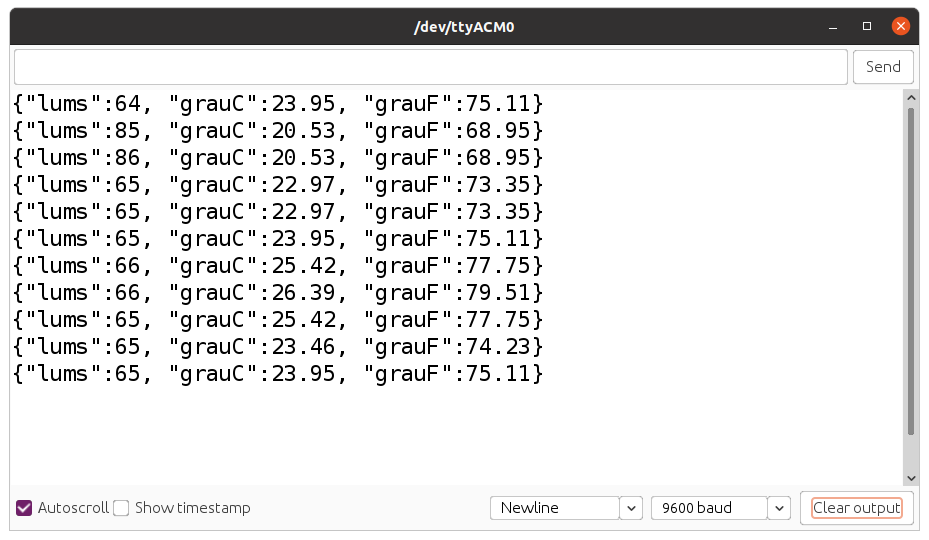
\includegraphics[width=0.50\textwidth]{images/saida}
	\caption{Saída da Serial}
\end{figure}

\textbf{NOTA}. Aqui estamos usando o tempo de 5 segundos apenas como característica de teste, mas na prática podemos aumentar para minutos pois não existe uma diferença muito grande de temperatura ou luminosidade em um intervalo de tempo em segundos. Qual o motivo de usamos um sensor de luminosidade juntamente como um de temperatura? Existe uma relação entre essas grandezas, e esse é o ponto de partida para uma interessante pesquisa podemos tentar explorar esse assunto em futuros trabalhos.

\section*{Banco de dados padrão SQL}
Esse tipo de Banco trabalha com SQL (Linguagem de Consulta Estruturada, do inglês \textit{Structured Query Language}) como interface. Normalmente Bancos de dados nesse padrão são conhecidos como SGBDR - Sistema de Gerenciamento de Banco de Dados Relacional (ou RDBMS do inglês Relational Database Manager System).

\subsection*{MySQL}
O primeiro banco de dados que utilizaremos é o MySQL. \textbf{MySQL} é um SGBDR gratuito e de código aberto. Seu nome é uma combinação de "My", o nome da filha do co-fundador Michael Widenius, e "SQL", a abreviação de \textit{Structured Query Language}. É atualmente um dos bancos mais populares, e atualmente pertence a \textit{Oracle Corporation}, com mais de 10 milhões de instalações pelo mundo. 

Após estar instalado corretamente em seu ambiente. Criamos um database: \\
{\ttfamily create database projetoint}

Este tipo de SGBDR utiliza databases para separar as tabelas e permitir uma melhor organização. Usamos esse database: \\
{\ttfamily use projetoint}

E criamos a seguinte entidade:
\begin{lstlisting}[]
CREATE TABLE dados (
  datahora timestamp NOT NULL,
  ldr int4 NOT NULL,
  tempC float8 NOT NULL,
  tempF float8 NOT NULL,
  CONSTRAINT ldr_pkey PRIMARY KEY (datahora)
);
\end{lstlisting}

Nossa entidade possui os campos: \textbf{datahora} como chave primária que contém a data e hora da coleta, \textbf{ldr} com o valor do sensor de luminosidade em uma escala de 0 a 100, \textbf{tempC} para o valor do sensor da temperatura em graus na escala Celsius e \textbf{tempF} para o valor do sensor da temperatura em graus na escala Farenheit.

Para que o Python possa se comunicar com o MySQL é necessário instalar a biblioteca \textbf{mysql-connector-python}: \\
{\ttfamily\$ python -m pip install mysql-connector-python}

Importamos as bibliotecas necessárias:
\begin{lstlisting}[]
import mysql.connector
import serial
import simplejson
from datetime import datetime
\end{lstlisting}

Criamos o seguinte método para gravar os dados no banco de dados:
\begin{lstlisting}[]
def gravar_dados(conn, JSON):
  try:
    cursor = con.cursor()
    cursor.execute("""
      INSERT INTO dados (datahora, ldr, tempC, tempF)
      VALUES (%(data)s, %(lums)s, %(grauC)s, %(grauF)s);
      """, JSON)
    con.commit()
    count = cursor.rowcount
    print(count, "Registro inserido com sucesso!")
  except (Exception) as error:
    print("Falhou para inserir registro!", error)
\end{lstlisting}

Essa função recebe a conexão com o banco e dado em formato JSON lido. Criamos um objeto cursor (a conversação com o MySQL é realizada através desse objeto). Executamos um \textbf{INSERT} no banco que monta os dados através do JSON passado. Damos um \textit{commit()} para gravar os dados, obtemos a resposta quantas linhas foram executadas com o comando, mostramos esse resultado e encerramos a conexão. Caso ocorra qualquer problema este será mostrado um erro pois existe uma proteção do código com um comando \textit{try-except}.

E o seguinte método para obter os dados do componente:
\begin{lstlisting}[]
  def ler_dados_serial():
    ser = serial.Serial('/dev/ttyACM0', 9600, timeout=5)
    con = mysql.connector.connect(
        host="localhost",
        user="root",
        password="root",
        database="projetoint"
    )    
    while True:
      try:
        ler = ser.readline()
        json = simplejson.loads(ler.decode('utf8').replace("'", '"'))
      except (Exception) as error:
        print("Falhou para ler registro!", error)
        continue
      dt_str = datetime.now().strftime("%Y/%m/%d %H:%M:%S")
      json["data"] = dt_str
      gravar_dados(con, json)

    ser.exit()
\end{lstlisting}

Iniciamos a variável \textbf{ser} com os dados da serial (lembrar que ao rodar esse programa, a janela \textbf{Serial Monitor} da Arduino IDE deve estar fechada para evitarmos conflito), são três indicações: a porta que o Arduino está ativo, a velocidade de leitura (que acertamos a 9.600 bounds) e o tempo que deve ser realizada a leitura (cada 5 segundos). 

Para a conexão criamos uma variável \textbf{con} que contém os seguintes valores: \vspace{-1em}
\begin{itemize}[nolistsep]
	\item \textbf{host} - servidor (IP) que se encontra o banco.
	\item \textbf{user} - o nome do usuário.
	\item \textbf{password} - senha desse usuário.
	\item \textbf{database} - o nome da base de dados.
\end{itemize}

Entramos em um laço que colherá os dados. Neste lemos o conteúdo da serial e o colocamos na variável \textbf{ler}, usamos um objeto da biblioteca \textit{simplejson} para converter seu conteúdo para o padrão JSON correto. Para obter os dados decodificamos a saída para o padrão UTF-8 (muitos sistemas Windows exigem essa cláusula, já no padrão Unix não existe essa necessidade). 

Adicionamos o campo \textbf{data} com o valor da data e hora atual (outro pulo do gato) sempre que for gravar data em um banco de dados use o formato \textbf{Y/M/D}. Os formatos \textbf{D/M/Y} e \textbf{M/D/Y} dependem de como está configurado o banco, já o formato \textbf{Y/M/D} não tem erro pois quando o primeiro valor possui 4 dígitos e o banco assume esse formato. 

Gravamos esse na base com uma chamada ao método anteriormente visto com a passagem da variável de conexão e o JSON da leitura. E agora basta disparar esse método na chamada principal:
\begin{lstlisting}[]
  if __name__ == '__main__':
    ler_dados_serial()
\end{lstlisting}

E podemos armazenar os dados de luminosidade e temperatura para um determinado ambiente. Outra dica interessante seria trocar o componente \textbf{LM35} (que mede apenas temperatura) por um sensor denominado \textbf{DHT11} (que além da temperatura mede também a umidade).

\subsection*{Postgres}
\textbf{PostgreSQL}, também conhecido como Postgres, é um SGBD (Sistema Gerenciador de Banco de Dados) relacional gratuito e de código aberto que enfatiza a extensibilidade e conformidade com padrão SQL. Seu nome refere-se às suas origens como sucessor do banco \textbf{Ingres} e desenvolvido na Universidade da Califórnia, em \textit{Berkeley}. Este deve estar instalado corretamente em seu ambiente. Por padrão do Postgres, estaremos alocados em um Database de mesmo nome.

Neste criamos um esquema: \\
{\ttfamily create schema projetoint}

Sempre que trabalhamos com bancos de dados que assim permitam é preferível usar um esquema para separar as tabelas e permitir uma melhor organização. E a seguinte entidade:
\begin{lstlisting}[]
CREATE TABLE projetoint.dados (
  datahora timestamp NOT NULL,
  ldr int4 NOT NULL,
  tempC float8 NOT NULL,
  tempF float8 NOT NULL,
  CONSTRAINT ldr_pkey PRIMARY KEY (datahora)
);
\end{lstlisting}

A entidade criada é a cópia exata como vimos para o MySQL. Para que o Python possa se comunicar com o Postgres é necessário instalar a biblioteca \textbf{psycopg2}: \\
{\ttfamily\$ pip install psycopg2-binary}

Importamos as bibliotecas necessárias:
\begin{lstlisting}[]
import psycopg2
import serial
import simplejson
from datetime import datetime
\end{lstlisting}

Criamos o seguinte método para gravar os dados no banco de dados:
\begin{lstlisting}[]
def gravar_dados(con, JSON):
  try:
    cursor = con.cursor()
    cursor.execute("""
      INSERT INTO projetoint.dados (datahora, ldr, tempC, tempF)
      VALUES (%(data)s, %(lums)s, %(grauC)s, %(grauF)s);
      """, JSON)
    con.commit()
    count = cursor.rowcount
    print(count, "Registro inserido com sucesso!")
    con.close()
  except (Exception) as error:
    print("Falhou para inserir registro!", error)
\end{lstlisting}

Comparando com a função já vista para o banco MySQL apenas o comando INSERT foi modificado para adicionarmos o esquema do banco. E o seguinte método para obter os dados do componente:
\begin{lstlisting}[]
  def ler_dados_serial():
    ser = serial.Serial('/dev/ttyACM0', 9600, timeout=5)
    con = psycopg2.connect(
        "host=localhost port=5432 dbname=postgres user=postgres password=postgres")    
    while True:
      try:
        ler = ser.readline()
        json = simplejson.loads(ler.decode('utf8').replace("'", '"'))
      except (Exception) as error:
        print("Falhou para ler registro!", error)
        continue
      dt_str = datetime.now().strftime("%Y/%m/%d %H:%M:%S")
      json["data"] = dt_str
      gravar_dados(con, json)

    ser.exit()
\end{lstlisting}

Novamente pouquíssimas modificações aqui somente quanto ao objeto de conexão \textbf{con} que contém os seguintes valores: \vspace{-1em}
\begin{itemize}[nolistsep]
	\item \textbf{host} - servidor (IP) que se encontra o banco.
	\item \textbf{port} - porta que se encontra o banco.
	\item \textbf{dbname} - o nome da base de dados.
	\item \textbf{user} - o nome do usuário.
	\item \textbf{password} - senha desse usuário.
\end{itemize}

Gravamos esse na base com uma chamada ao método anteriormente visto com a passagem da variável de conexão e o JSON da leitura. E agora basta disparar esse método na chamada principal:
\begin{lstlisting}[]
  if __name__ == '__main__':
    ler_dados_serial()
\end{lstlisting}

O que percebemos é todo banco SQL processa a inclusão dos valores praticamente de mesmo modo, sendo necessário mudar o conector e adaptar a instrução SQL de forma correta.

\section*{Bancos de Dados NoSQL}
Existem quatro tipos de bancos no padrão NoSQL, não pretendo aqui debater a vantagem de cada um deles, vamos realizar as modificações necessárias no programa em Python possa se utilizar um de cada tipo.

\subsection*{MongoDB - Tipo: Orientado a Documento}
Para gravarmos os dados necessitamos da biblioteca "pymongo" que pode ser instalada com o comando: \\
{\ttfamily\$ pip install pymongo}

Importamos essa biblioteca para o programa:
\begin{lstlisting}[]
from pymongo import MongoClient
\end{lstlisting}

E no método \textit{gravar\_dados()} modificar para a seguinte codificação:
\begin{lstlisting}[]
  def gravar_dados(json):
    cliente = MongoClient("localhost", 27017)
    db = cliente['coleta']
    col = db['dados']
    chv = col.insert_one(json)
    print("Registro Inserido: ", chv.inserted_id)
    cliente.close()	
\end{lstlisting}

Realizamos a conexão com o banco de dados que deve estar disponível na porta 27017, criamos ou abrimos a base "coleta" e a coleção "dados" e inserimos o registro do JSON enviado através do comando \textbf{insert\_one}, essas três linhas poderiam ser reescritas para: \\
{\ttfamily cliente['coleta']['dados'].insert\_one(json)}

Porém para facilitar o entendimento deixamos com três objetos. Mostramos a chave do registro inserido e encerramos a conexão.

\subsection*{Redis - Tipo: Orientado a Chave-Valor}
Para gravarmos os dados necessitamos da biblioteca "redis" que pode ser instalada com o comando: \\
{\ttfamily\$ pip install redis}

Importamos essa biblioteca para o programa:
\begin{lstlisting}[]
import redis
\end{lstlisting}

E no método \textit{gravar\_dados()} modificar para a seguinte codificação:
\begin{lstlisting}[]
  def gravar_dados(json):
    r = redis.Redis(host='localhost', port='6379')
    with r.pipeline() as pipe:
      chave = json["data"]
      pipe.hset(chave, "ldr", json["lums"])
      pipe.hset(chave, "tempC", json["grauC"])
      pipe.hset(chave, "tempF", json["grauF"])
      pipe.execute()
    r.bgsave()
    r.close()
\end{lstlisting}

De modo extremamente simples, criamos uma conexão com o banco, e usamos a técnica de pipeline para que possamos gravar um registro chave-valor com subcampos chave-valor. O dado de \textbf{datahora} será a chave principal do registro (pois esse nunca se repete), e gravamos os outros 3 campos obtendo os dados do arquivo JSON e enviando-os para o padrão chave-valor do Redis.

\subsection*{Neo4j - Tipo: Orientado a Grafo}
Para gravarmos os dados necessitamos da biblioteca "neo4j" que pode ser instalada com o comando: \\
{\ttfamily\$ pip install neo4j}

Importamos essa biblioteca para o programa:
\begin{lstlisting}[]
from neo4j import GraphDatabase
\end{lstlisting}

Adicionamos uma constante que vai manter nosso comando \textit{Cypher} para criar o registro, abaixo das importações de bibliotecas:
\begin{lstlisting}[]
cqlCriar = "CREATE (:coleta { data: $data, ldr: $ldr, tempC: $tempC, tempF: $tempF})"	
\end{lstlisting}

E modificamos o método \textit{gravar\_dados()}:
\begin{lstlisting}[]
  def gravar_dados(json):
    graphDB_Driver = GraphDatabase.driver(
      "bolt://localhost:7687", auth=("neo4j", "test"))
    with graphDB_Driver.session() as secao:
      secao.run(cqlCriar, data=json["data"],
        ldr=json["lums"], 
        tempC=json["grauC"], 
        tempF=json["grauF"])
      secao.close()
\end{lstlisting}

Criamos uma conexão com o banco, e abrimos uma seção para essa conexão. Em seguida executamos o comando \textit{Cypher} e adicionamos a cada parâmetro (iniciado por {\ttfamily\$}) o seu respectivo valor obtido através do JSON. E encerramos a seção aberta.

\subsection*{Apache Cassandra - Tipo: Orientado a Coluna}
Antes de qualquer atividade no Python precisamos acessar o \textbf{CQL} do banco Apache Cassandra para digitarmos os seguintes comandos para criarmos \textit{KeySpace}: \\
{\ttfamily cqlsh> CREATE KEYSPACE coleta WITH replication = \{'class':'SimpleStrategy', \\ 'replication\_factor':1\};} 

E a tabela que receberá os dados: \\
{\ttfamily cqlsh> use coleta;} \\
{\ttfamily cqlsh:coleta> CREATE TABLE dados (datahora timestamp PRIMARY KEY, ldr int, \\ tempC float, tempF float);}

Para gravarmos os dados necessitamos da biblioteca "cassandra-driver" que pode ser instalada com o comando: \\
{\ttfamily\$ pip install cassandra-driver}

Através dessa biblioteca importamos 2 objetos que utilizaremos:
\begin{lstlisting}[]
from cassandra.cluster import Cluster
from cassandra.query import SimpleStatement
\end{lstlisting}

Adicionamos novos métodos, pois a coluna \textit{timestamp} trabalha com elementos do tipo inteiro longo:
\begin{lstlisting}[]
  def unix_time(dt):
    epoch = datetime.utcfromtimestamp(0)
    delta = dt - epoch
    return delta.total_seconds()
	
  def unix_time_millis(dt):
    return int(unix_time(dt) * 1000.0)
\end{lstlisting}

No método \textit{ler\_dados\_serial()} adicionamos os objetos para nos conectarmos ao Cassandra:
\begin{lstlisting}[]
  def ler_dados_serial():
	ser = serial.Serial('/dev/ttyACM0', 9600, timeout=4)
	session = Cluster().connect()
	session.execute("USE coleta;")
\end{lstlisting}

Passamos este na chamada ao método \textit{gravar\_dados()}:
\begin{lstlisting}[]
	gravar_dados(session, json)
\end{lstlisting}

E na montagem do elemento \textit{data} para o JSON, realizamos a seguinte modificação:
\begin{lstlisting}[]
	dt_long = unix_time_millis(datetime.now())
	json["data"] = dt_long
\end{lstlisting}

E modificamos o método \textit{gravar\_dados()}:
\begin{lstlisting}[]
  def gravar_dados(session, JSON):
    try:
      session.execute("""
        INSERT INTO dados (datahora, ldr, tempC, tempF)
        VALUES (%(data)s, %(lums)s, %(grauC)s, %(grauF)s);""", JSON)
      print("Registro inserido com sucesso!")
    except (Exception) as error:
      print("Falhou para inserir registro!", error)
\end{lstlisting}

E agora podemos escolher qual base de dados seja padrão SQL ou NoSQL se encaixa melhor para o projeto que estamos realizando.
\end{document}